%
% Chapter 3
%

\chapter{LHC and the CMS detector}
\label{chap:exper_setup}

\section{Introduction}

The prime goals of the LHC and the Compact Muon Solenoid (CMS) \cite{Chatrchyan:2008aa} experiment are exploring the physics at the TeV scale and studying the mechanism of electroweak symmetry breaking, including studying the SM Higgs boson properties along with searches for new particles predicted by beyond the SM physics. The physics program's other main interests include studies of the SM top quark properties, electroweak physics, and physics of hadrons containing a charm or bottom quark. Heavy-ion collisions address the physics of strongly interacting matter and the quark-gluon plasma. Hadrons consist of quark and gluons; therefore, two colliding partons' initial energy is not known. In contrast, the collision's energy is known at lepton colliders, where each particle has the same energy. Thus, hadron colliders can explore a wide range of collision energies, while lepton colliders are well suited for precision measurements.

\section{The Large Hadron Collider}
\label{sec:LHC}

The LHC is a hadron accelerator located at CERN. The design was intended to collide proton beams with a beam energy of 7 TeV leading to a center-of-mass energy \sqs of 14 TeV and reach a luminosity of $10^{34} \lumi$. Lead (Pb) ions can be accelerated up to an energy of 2.8 TeV per nucleon and reach a luminosity of $10^{27} \lumi$. LHC is the most powerful tool for particle physics research that is currently available. The 26.7 km tunnel constructed between 1984 and 1989 for the Large Electron-Positron collider (LEP) \cite{Electron-Positron:1997351} was reused to install the LHC. There are eight arcs and eight straight sections lying 45-170 m below the surface. Unlike particle-antiparticle colliders that can use a single ring for both beams, the LHC uses two rings with counter-rotating beams. There is less synchrotron radiation owing to the heavier particles being collided at the LHC.

The accelerator complex acts as an injector of the protons and heavy ions. Protons are obtained from hydrogen gas after the electrons are stripped off, and they enter the Linear accelerator 2 (Linac2) \cite{accelerator:1997427}, where they are accelerated to 50 MeV. They are further accelerated in the Proton Synchrotron Booster (PSB) \cite{Synchrotron:1997372} to 1.4 GeV. They are then injected in the Proton Synchrotron (PS) \cite{Synchrotron:1997189}, where they are accelerated to 25 GeV. A bunch train is produced within the PS before extraction. The protons are then accelerated in the Super Proton Synchrotron (SPS) \cite{Synchrotron:1997188} to 450 GeV before injecting in the LHC.

The four interaction points are equipped with particle detectors: the CMS experiment, A Toroidal LHC ApparatuS (ATLAS) experiment \cite{Aad:2008zzm}, A Large Ion Collider Experiment (ALICE) \cite{Aamodt:2008zz}, and a Large Hadron Collider beauty (LHCb) \cite{Alves:2008zz} experiment. Two further smaller experiments, a Total, Elastic, and diffractive cross section Measurement (TOTEM) \cite{Anelli:2008zza} and the Large Hadron Collider forward (LHCf) \cite{Adriani:2008zz} experiment, are located near the CMS interaction point and near the ATLAS interaction point, respectively.

The ATLAS and CMS experiments have both multi-purpose detectors installed. The detectors were build to detect particles from proton-proton (p-p) or heavy-ion (Pb-Pb) collisions. One of the main tasks currently is to study the production and decay of the discovered Higgs boson \cite{Chatrchyan:2013lba}, disentangle its properties, and check if it is the SM Higgs boson or a Higgs boson of an extension of the SM. The other tasks involve high precision tests of QCD, electroweak interactions, and heavy flavor physics. Precision measurements of production, the couplings, and the spin of the top quark are also pursued. Several searches for supersymmetric particles and Dark Matter are also ongoing.

During the LHC Run II data-taking, a bunch spacing of 25 ns was used, and proton-proton collision data were collected at $\sqs = 13$ TeV in 2016, 2017, and 2018. The integrated luminosity delivered to CMS as a function of time is shown in Figure \ref{fig:lumi} for each proton-proton collision data-taking period. CMS does not record the whole delivered data, and only part of the recorded that is considered good is used for physics analysis.

\begin{table}[!hbpt]
  \centering
  \caption{Integrated luminosity considered for physics analysis at the CMS experiment during Run II}
  \begin{tabular}{|c|c|}
    \hline Year & Integrated luminosity \\
    \hline 2016 & $35.9 \fb$ \\
    \hline 2017 & $41.5 \fb$ \\
    \hline 2018 & $59.3 \fb$ \\
    \hline
  \end{tabular}
  \label{tab:luminosity}
\end{table}

\begin{figure}[htbp]
  \centering
  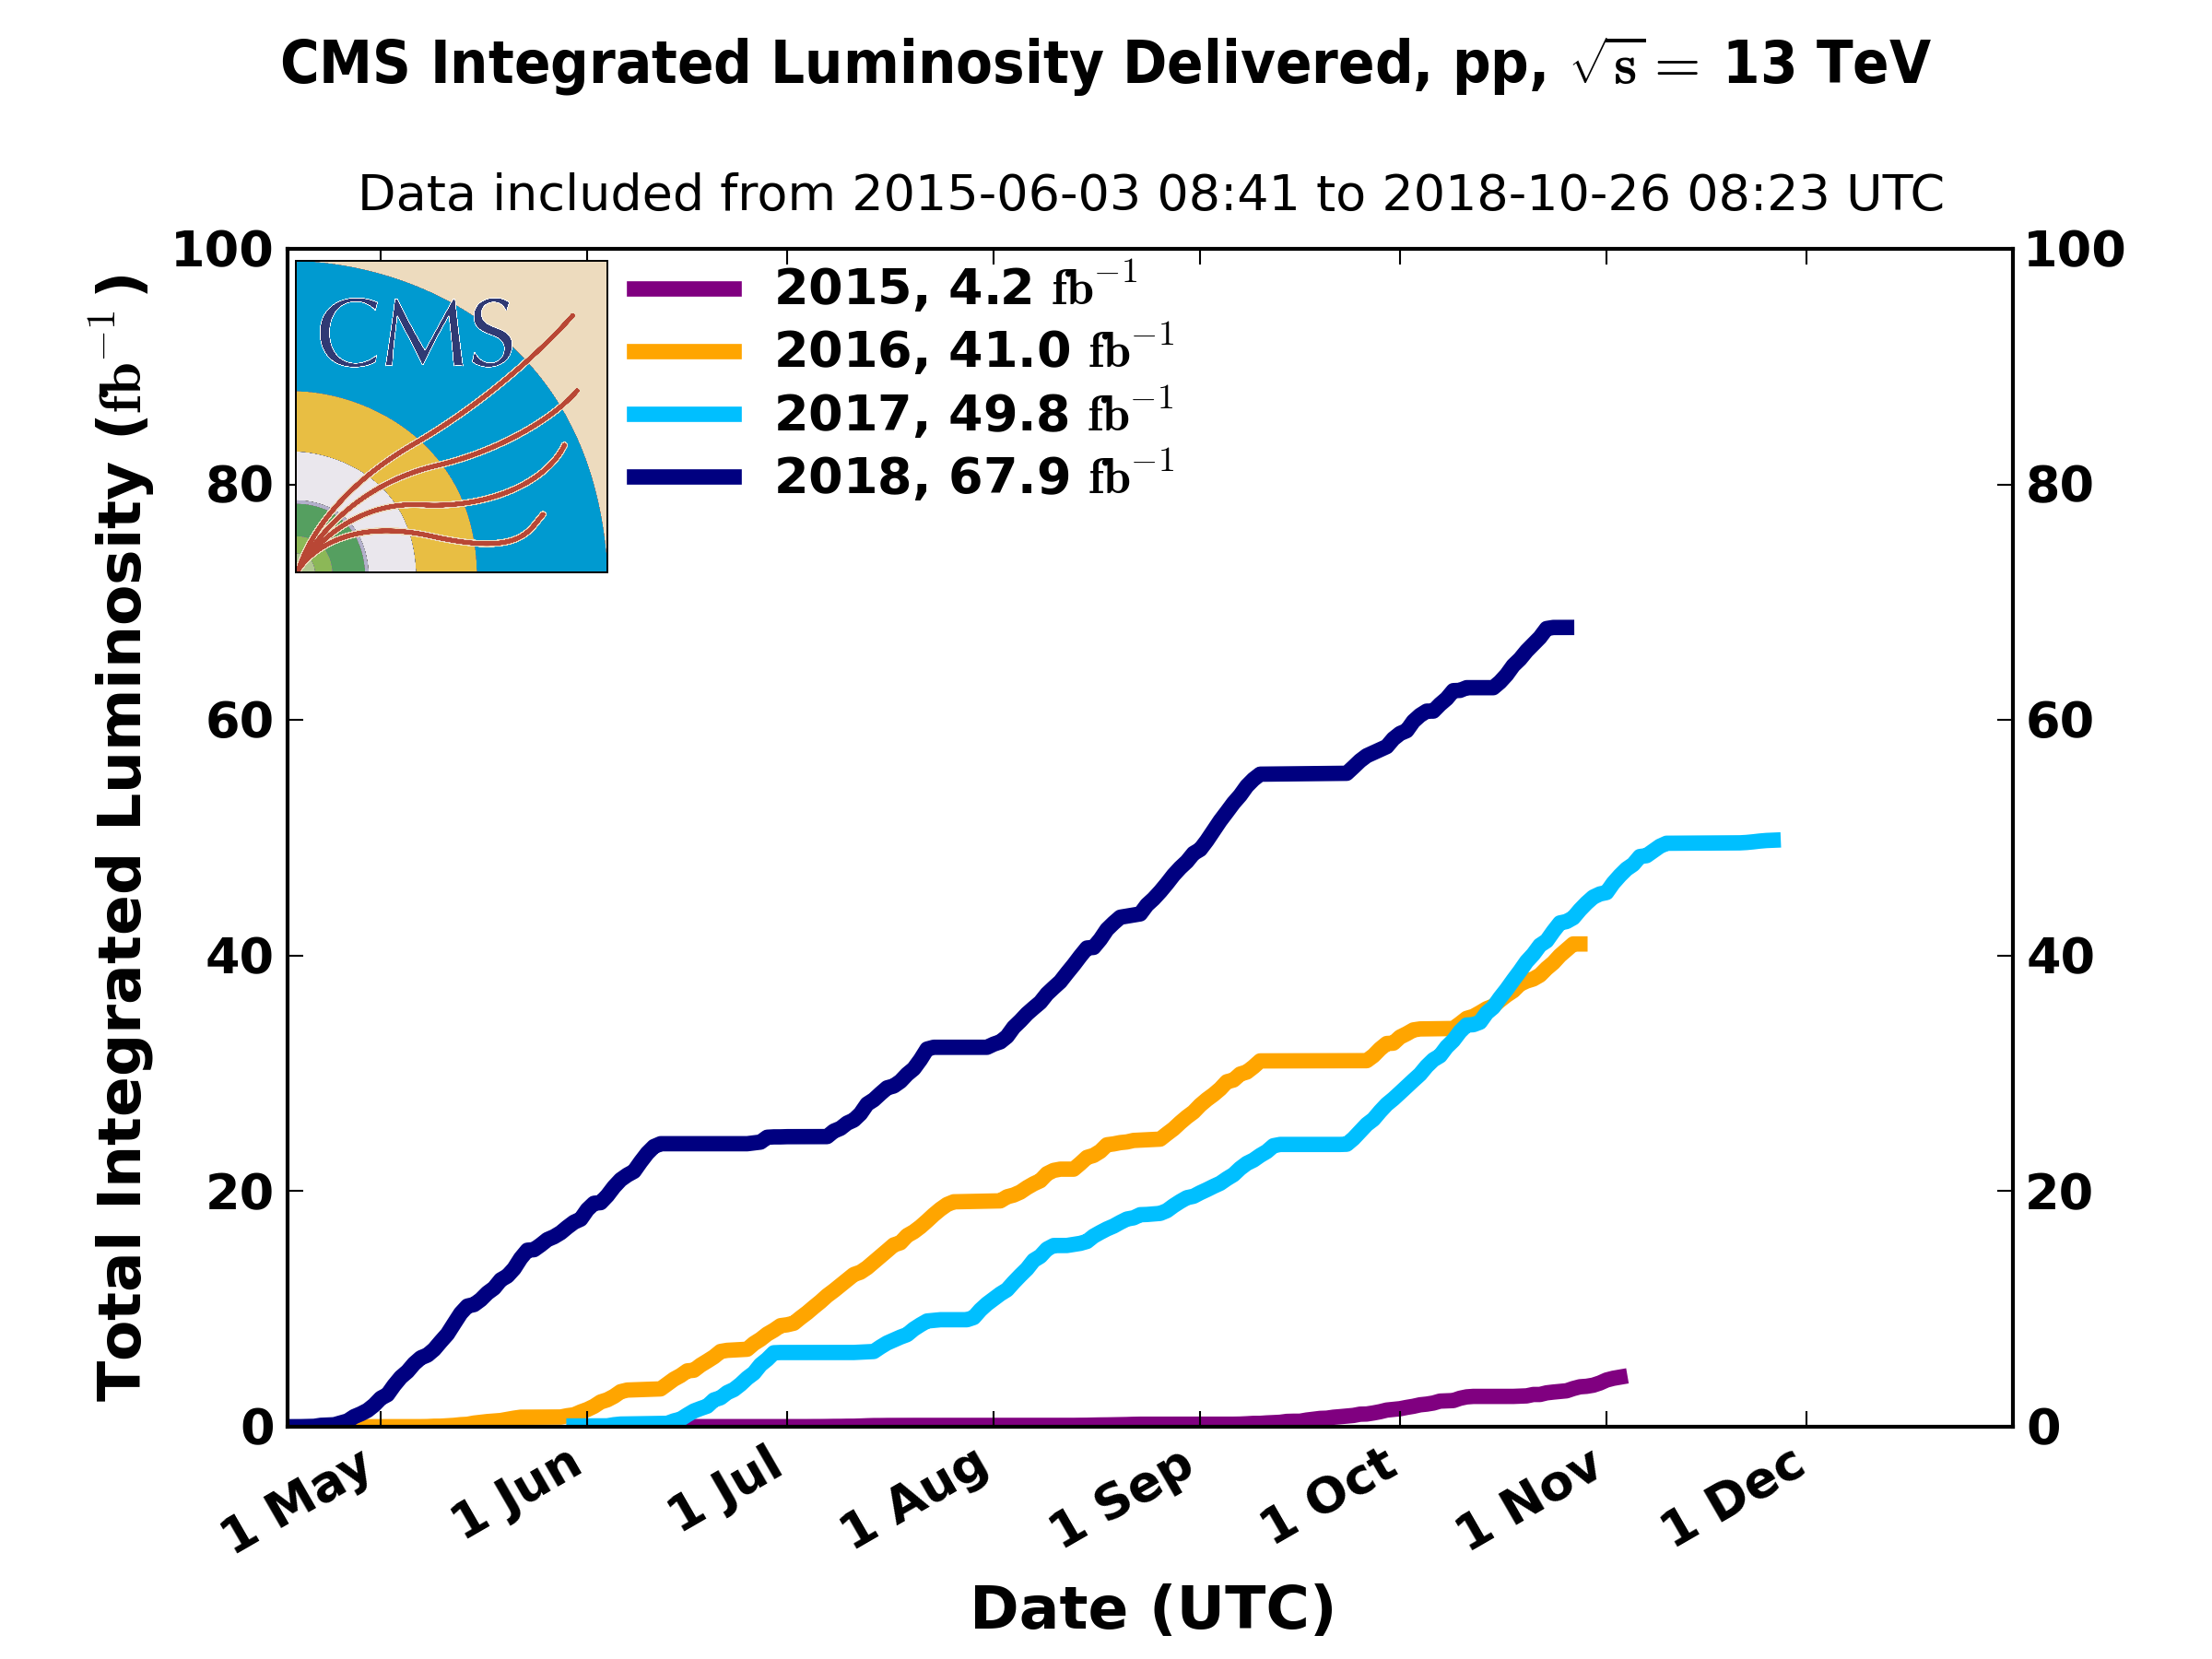
\includegraphics[width=0.8\textwidth]{plots/chapter3/int_lumi.png}
  \caption{Cumulative luminosity as a function of time delivered to CMS during stable beams for proton-proton collisions. The luminosity is shown for 2015 (purple), 2016 (orange), 2017 (light blue), and 2018 (dark blue). \cite{lumi}}
  \label{fig:lumi}
\end{figure}

\section{The Compact Muon Solenoid experiment}
The layout of the CMS detector is shown in Figure \ref{fig:cms}. As the name ``Compact Muon Solenoid'' indicates, a superconducting solenoid is the heart of CMS. Considerable bending power for the momentum measurement of charged particles within a compact design is achieved using a high magnetic field of 3.8 T. The internal part of the magnetic coil is large enough to accommodate the inner tracking system and the calorimetry. The inner tracking system is composed of a pixel detector close to the interaction region and a silicon strip tracker. The pixel detector can resolve individual vertices and distinguish between vertices from the primary interaction and secondary vertices from the decay of the primary interaction particles. Trajectories are precisely measured with the high granular silicon strip tracker, which can deal with high charged particle multiplicities.

\begin{figure}[htbp]
  \centering
  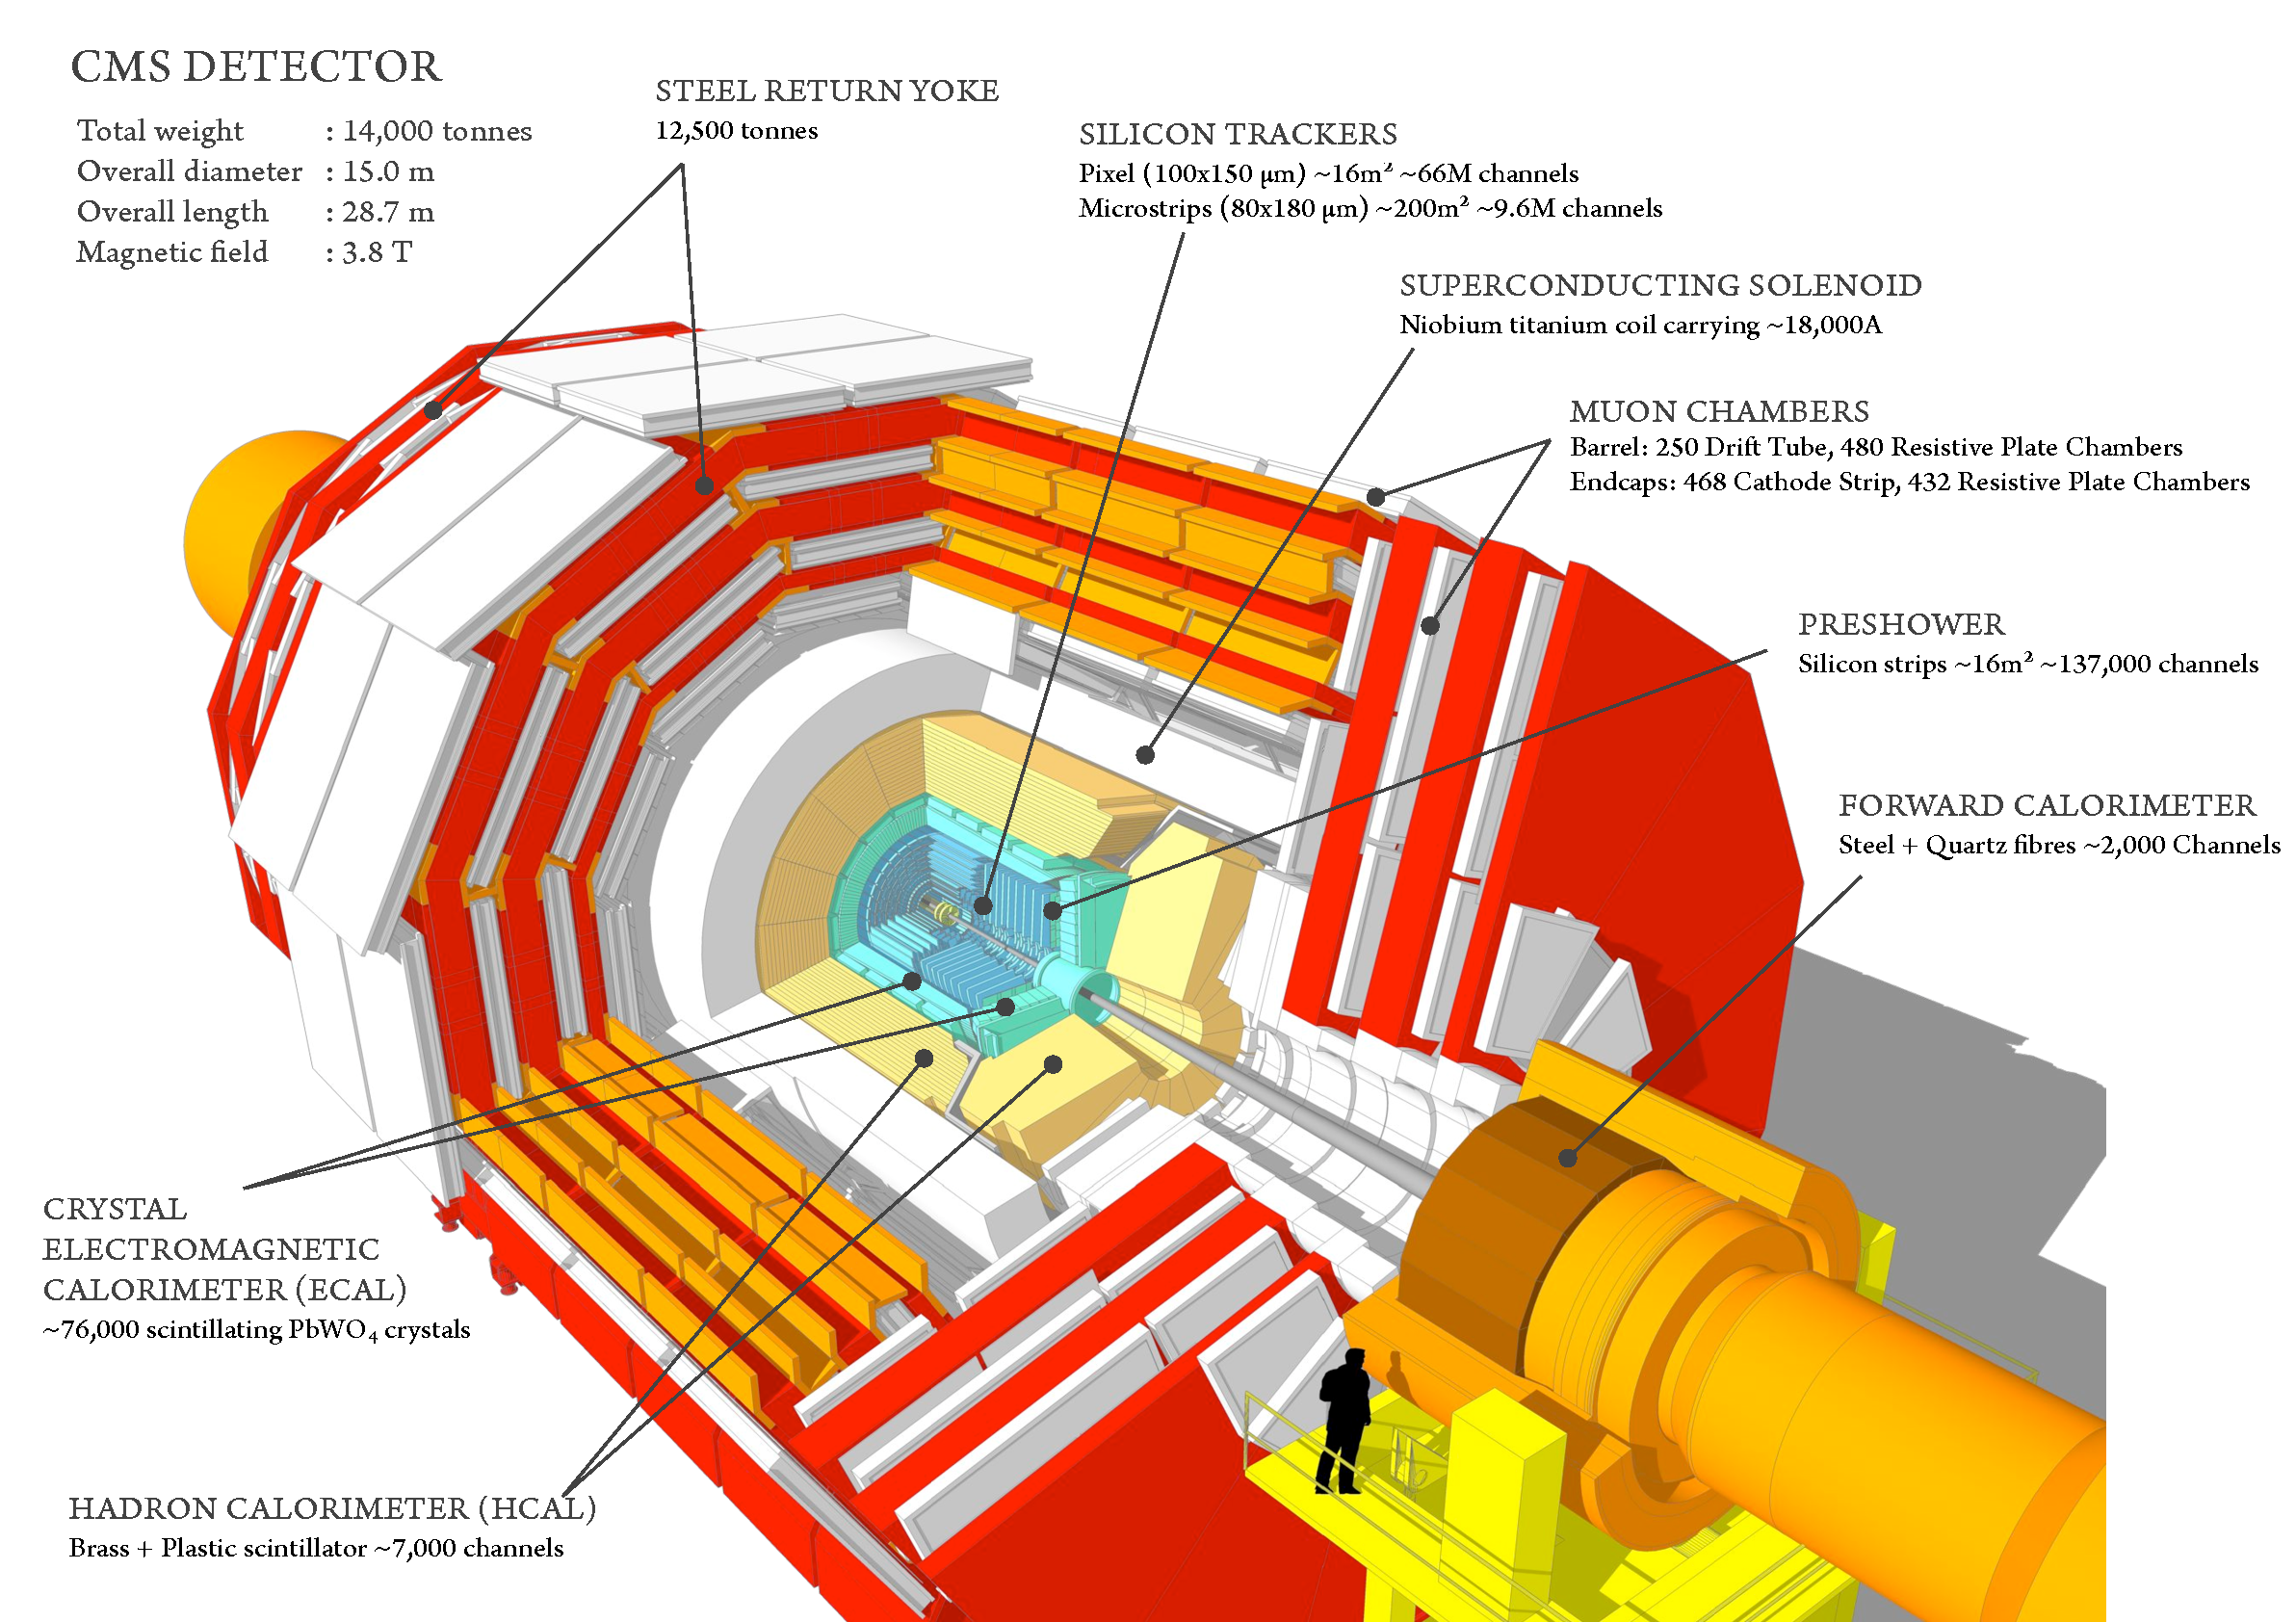
\includegraphics[width=0.9\textwidth]{plots/chapter3/cms_layered.png}
  \caption{Schematic view of the CMS detector.}
  \label{fig:cms}
\end{figure}

The energy of the particles is measured in calorimeters. Calorimeter material initiates electromagnetic (EM) or hadronic showers. For electromagnetic interactions, the characteristic interaction length is the radiation length $X_0$, while the characteristic interaction length for hadronic showers is the nuclear interaction length $\lambda_I$. The entire volume is sensitive in homogeneous calorimeters, while sampling calorimeters consist of metallic absorber sandwiched or threaded with an active material that generates the signal. CMS has an EM calorimeter (ECAL) made of lead tungstate $PbWO_{4}$ in front of a brass/scintillator sampling hadron calorimeter (HCAL). An additional layer of scintillators is outside the coil. The magnet is used as an absorber material. This iron/quartz-fiber calorimeter is referred to as the hadron outer (HO) detector. The muon detectors are sandwiched between the layers of the steel return yoke. Their main task is to trigger on muons and to identify the muons with good momentum resolution.

\subsection{The coordinate system of CMS}
CMS uses a right-handed Cartesian coordinate system with its origin at the detector's center, the nominal interaction point. The x-axis points towards the LHC center, while the y-axis points upward towards the surface and perpendicular to the LHC plane. Thus, the z-axis points along the anticlockwise beam-direction. Two angles are defined, where the azimuthal angle $\phi$ is measured from the x-axis in the x-y plane, and the polar angle $\theta$ is measured from the z-axis. Pseudorapidity is defined as

\begin{equation}
  \eta=-\ln \left[\tan \left(\frac{\theta}{2}\right)\right]
\end{equation}

and describes the angle of a particle relative to the beam axis, illustrated in Figure \ref{fig:coordinate}. Distances in $\phi$ and $\eta$ are denoted $\Delta\phi$ and $\Delta\eta$. These distance measures are used to define the spatial separation between physics objects by $\Delta R$ with

\begin{equation}
  \Delta \mathrm{R}=\sqrt{(\Delta \phi)^{2}+(\Delta \eta)^{2}}
\end{equation}

\begin{figure}[htbp]
  \centering
  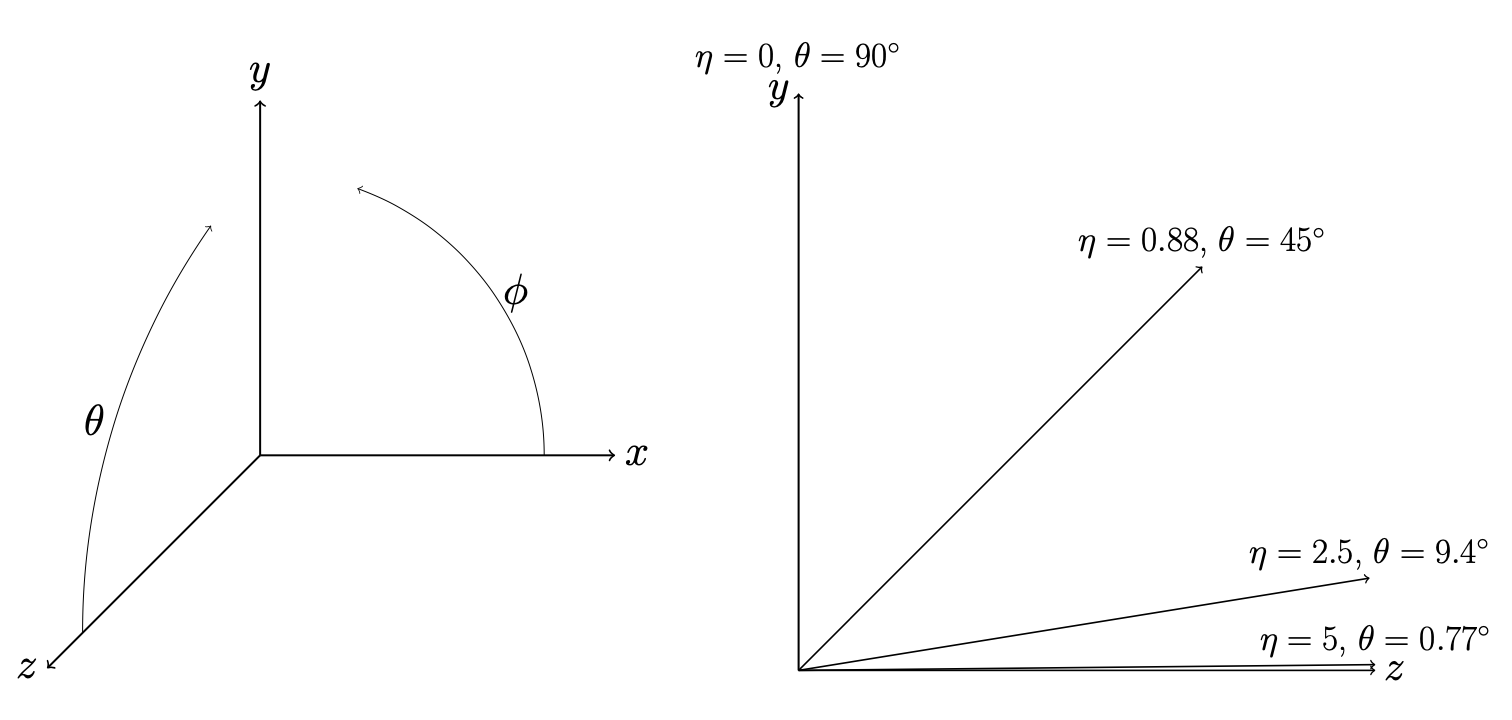
\includegraphics[width=0.9\textwidth]{plots/chapter3/coordinate.png}
  \caption{Coordinate system convention of CMS (left) and the relation between pseudorapidity $\eta$ and polar angle $\theta$ (right)}
  \label{fig:coordinate}
\end{figure}

\subsection{Kinematic quantities}
At LHC, the protons carry half of the collision energy \sqs. The hard interactions do not take place between the colliding protons but between two of their partons. Each parton carries a fraction of $x_i$ of the proton momentum. As the parton mass can be neglected with respect to the momentum $\vec{p}$, the parton energy is given by its momentum. In the laboratory frame, the four-momenta of the partons are

\begin{equation}
  \mathrm{p}_{1}=x_{1} \cdot \frac{\sqs}{2}(1,0,0,1) \\
  \mathrm{p}_{2}=x_{2} \cdot \frac{\sqs}{2}(1,0,0,-1)
\end{equation}

Then, the invariant mass M of the hard collision is given by

\begin{equation}
  \hat{s} \equiv \mathrm{M}^{2}=\left(\mathrm{p}_{1}+\mathrm{p}_{2}\right)^{2}=\frac{s}{4} \cdot\left[\left(x_{1}+x_{2}\right)^{2}-\left(x_{1}-x_{2}\right)^{2}\right]=x_{1} x_{2} s
\end{equation}

where $\sqrt{\hat{s}}$ denotes the center-of-mass energy of the parton-parton collision. The hard collision products have a total momentum, zero for the x- and y-components but in general non-zero for the z-component. Thus, the hard-collision products' momentum and energy are measured transverse to the beam direction in the x-y plane. \pt and \ET denote the transverse momentum and transverse energy respectively, with $\ET = \text{E} \cdot \text{sin} \theta$. Only weakly interacting particles, such as neutrinos, do not produce a signal in the CMS detector and lead to an imbalance in the observed total transverse momentum in the event, missing transverse energy, denoted as \met.

\subsection{Detector requirements}
Final states that contain isolated leptons and photons leave clean signatures in the CMS detector. A good muon identification and momentum resolution are needed over a wide range of momenta. The muon charge has to be determined unambiguously. Furthermore, a good momentum resolution and reconstruction efficiency of charged particles are crucial for reconstructing electrons and charged hadrons. Charged-particle momenta are measured using the curvature of their trajectory. Considerable bending power is needed to measure precisely the momentum of particles with large momentum. Additionally, a good electromagnetic energy resolution is needed with wide geometrical coverage. The direction of the photons and correct localization of the primary interaction should be measurable.

Quarks hadronize, and the hadrons can be detected with the CMS detector. Good identification of hadronically decaying taus is needed for the Higgs boson physics. The triggering and identification efficiency of hadronically decaying taus can be improved by a good measurement of the impact parameter of charged-particle tracks and good position measurement of the secondary vertices. This requires pixel detectors close to the interaction region. Hadronic calorimeters with a large hermetic coverage ($|\eta| < 5$) and with a fine lateral segmentation $(\Delta \eta \times \Delta \phi<0.1 \times 0.1)$ are required for a good energy measurement of hadrons and estimation of \met.

The collisions are happening at a rate of $40 \mathrm{MHz}$ and not all of these events can be stored; therefore, only interesting events have to be selected. The online event selection process, trigger, must reduce the rate to no more than a few hundred events per second. The short time between two bunch crossings, 25 ns, has a major implication on the readout and trigger system design. Multiple proton-proton interactions (pileup) happen in one bunch crossing. The interactions' products overlap and can be wrongly linked. Long response times of detector elements and their electronic signal longer than 25 ns increase this effect. High granularity detectors with good time resolution result in a low occupancy. This requires many detector channels and, therefore, a good synchronization of the electronic detector channels. The large flux of the particles and resulting high radiation levels require radiation-hard detectors and front-end electronics.

\subsection{Magnet}

The curvature of the particle trajectory in a magnetic field determines the momenta and sign of charged particles. The most important aspect of muon measurement is the choice of magnetic field configuration. A good momentum resolution of $\Delta \mathrm{p} / \mathrm{p} \approx 10 \%$ is required for muons with a momentum of 1 TeV. CMS uses a large superconducting solenoid with a magnetic field of 3.8 T. The solenoid is 13 m long and has an inner diameter of 5.9 m. The superconductor material is Niobium titanium \cite{BUL-NA-2003-150}. A high-purity aluminum-stabilized conductor with a four-layer winding is used, which has to withstand outward pressure. The conductor is composed of five coils, and its superconducting wire is cooled using an indirect cooling by thermosyphon.

\subsection{Inner Tracking system}

The inner tracking system \cite{Khachatryan:2010pw} measures the trajectories of particles up to $|\eta| < 2.5$. The particle flux is the highest close to the interaction region. The silicon pixel detector is placed close to the interaction region. This allows for the reconstruction of vertices from heavy flavor hadrons with a b or c quark. Each pixel has a size of $\approx 100 \times 150 \mum^{2}$. The spatial resolution of the radius and azimuthal angle $r-\phi$ measurement is about 10 $\mu m$, and 20 $\mu m$ for the z-coordinate measurement. In the intermediate region ($20 < r < 55$ \cm) and outermost region ($r > 55$ \cm) silicon microstrips are used with a size of $10 \cm \times 80 \mum$ (minimum cell size) and a size of $25 \cm \times 180 \mum$ (maximum cell size), which provide the required granularity. The barrel's tracking volume has a cylinder shape with a length of 5.8 m and a diameter of 2.6 m. The pixel detector consists of three layers at radii of 4, 7, and 11 \cm in the barrel.

Additionally, there are ten layers of silicon microstrip detectors. The strip tracker is divided into a Tracker Inner Barrel (TIB) made out of four layers and a Tracker Outer Barrel (TOB) made out of six layers. Each part has two layers which provide a single-point measurement in the $r - \phi$ and $r - z$ coordinates. In the TIB, the single-point resolution is $23 - 34 \mum$ in the r-direction and $23 \mum$ in z, while it is $35 - 52 \mum$ in the $r-\phi$ direction and $52 \mum$ in $z$ for the TOB. In the two end caps, there are just two-pixel layers and nine microstrip layers. The strip tracker's endcaps are divided into the Tracker End Cap made of 9 disks and the Tracker Inner Disks (TID), which are made of three small disks, which fill the gap between the TIB and the TEC.

\subsection{Electromagnetic Calorimeter}

The electromagnetic calorimeter (ECAL) measures the energy of electrons and photons. A hermetic, homogeneous crystal (ECAL) with a coverage of $|\eta| < 3$ is used, which has an excellent energy resolution and high granularity; therefore, it also has excellent separation of close clusters \cite{CMS:2010bta, Khachatryan:2015hwa}. It is used to identify photons, which leave no signal in the inner tracking detector. Lead tungstate ($PbWO_4$) crystals are used, which have a short radiation length of $X_0 = 0.89$ \cm, are radiation hard, and emit blue-green scintillation light with a maximum at 420 nm. The scintillation decay time is short and in the same order as the LHC bunch crossing time. About 80\% of the light is emitted within 25 ns. However, the light output depends on the temperature; therefore, a cooling system is needed to preserve the energy resolution. Furthermore, a low light yield requires photodetectors with intrinsic gain that can also operate in a high magnetic field. The crystals allow a compact calorimeter inside the solenoid that is fast, has a fine granularity, and is radiation-resistant. Figure \ref{fig:ecal} illustrates the layout of the CMS ECAL. The calorimeter is divided into a barrel ECAL (EB) which covers the region $0 < |\eta| < 1.479$ and two ECAL endcaps (EE) which cover the region $1.479 < |\eta| < 3.0$. Preshower detectors (ES) are installed in front of each endcap and cover the region $1.653 < |\eta| < 2.6$. In the EB, silicon avalanche photodiodes (APDs) are installed to detect the scintillation light. They also respond to temperature changes; therefore, they require a stable temperature.

\begin{figure}[htbp]
  \centering
  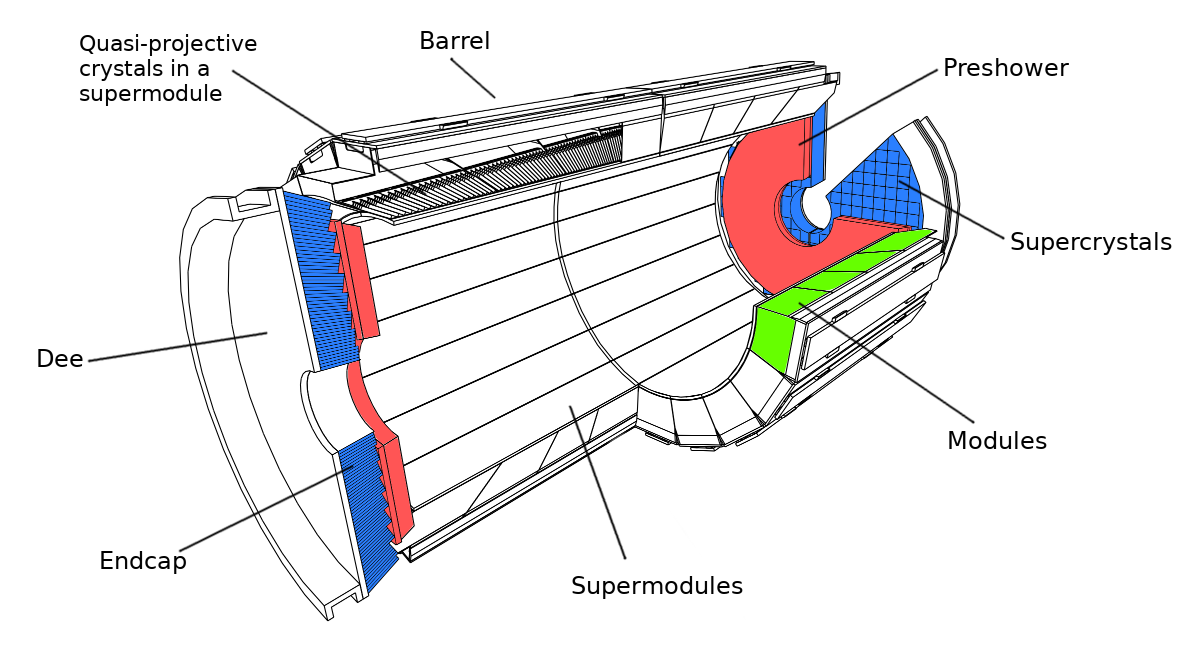
\includegraphics[width=0.9\textwidth]{plots/chapter3/ecal.png}
  \caption{Schematic view of the electromagnetic calorimeter.}
  \label{fig:ecal}
\end{figure}

The barrel section is structured in 36 identical supermodules, 18 in each half barrel, with the crystals being arranged in a grid and covering $\Delta \eta \times \Delta \phi=0.0174 \times 0.0174$. Vacuum phototriodes (VPTs) are installed in both EE for detecting the scintillation light. The crystals are arranged in units of $5 \times 5$ crystals termed super crystals (SC). Both the crystals and the SCs, are arranged in a rectangular x-y grid. Neutral pions dominantly decay to two photons. Two closely separated photons can mimic high-energy photons; therefore, a preshower system is installed in front of each EE to identify and reject $\pi^0$ mesons. It also improves the position determination of electrons and photons as it has a higher granularity than the EE. The preshower detector is a sampling calorimeter consisting of two layers of a lead absorber, which initiate the electromagnetic showers from incoming electrons or photons. Each lead radiator is followed by silicon strip sensors measuring the energy deposits and the transverse shower profiles. The strips in both planes of silicon sensors are orthogonal oriented and are placed after a radiation length of 1 $X_0$ and 2 $X_0$ of the lead absorber.

\subsection{Hadron Calorimeter}
The energy of hadrons is measured in the hadron calorimeter (HCAL). Most of the HCAL calorimetry is located inside the magnetic coil surrounding the ECAL system. An important requirement on the HCAL design is to minimize the non-Gaussian tails in the energy resolution and to provide a good hermeticity for the determination of \met. It is designed to maximize the interaction length of the material within the magnet coil. On the other hand, the amount of space devoted to the active medium is minimized. The HCAL is a sampling calorimeter which is divided into a hadron barrel (HB) detector, covering the region $|\eta| < 1.4$ and two hadron endcap (HE) detectors, covering $1.3 < |\eta| < 3.0$. Brass is used as an absorber material. Brass has a reasonably short interaction length, is easy to machine, and it is non-magnetic. A tile/fiber technology made of plastic scintillator tiles is used as an active medium. For the innermost and the outermost layer, stainless steel is used for structural strength. The 3.7-mm-thick scintillator plates are sandwiched between the absorber plates. Wavelength-shifting (WLS) fibers, embedded in the scintillator tiles, convert the scintillation light. Then, it is channeled to photodetectors via optical fibers. Multi-channel hybrid photodiodes (HPDs) detect the light. They can operate in high axial magnetic fields. The HB is read out as a single longitudinal sampling with a segmentation $\Delta \eta \times \Delta \phi=0.087 \times 0.087 \approx 5^{\circ} \times 5^{\circ}$, which are termed tower. In the HE, the $\phi$ segmentation is $5^{\circ} - 10^{\circ}$ and the $\eta$ segmentation is $0.087 - 0.35$ depending on $\eta$.

Additional layers of scintillators are installed outside the coil within the return yoke using the iron as an absorber—the sample energy from hadron showers, which leak through the rear of the calorimeters. The central shower containment and the \met resolution of the calorimeter are thus improved. This sampling calorimeter is referred to as Hadron Outer (HO) detector. It is located along with the barrel muon system; therefore, its segmentation closely follows the barrel muon system. It is divided into five sections along with $\eta$ termed rings. The HO follows the HCAL barrel geometry in $\eta$ and $\phi$ and covers the region $|\eta| < 1.26$. Two further detectors, which cover the region $2.9 < |\eta| < 5.0$, are not shown. They are specialized in measuring energetic forward hadronic showers and ensuring full geometric coverage for the transverse energy measurement. The Hadron Forward (HF) sampling calorimeters use steel as absorber material and quartz fibers as the active medium, which run parallel to the beam. Shower particles in the quartz emit Cherenkov light fibers. This light is channeled by the fibers to photomultipliers. There are two types of quartz fibers, long ones (1.65 m) and short ones (1.43 m). Neutral components of the hadron showers are preferentially sampled in the HF, leading to narrower and shorter hadronic showers. This is ideally suited for the forward region. The towers in HF have a segmentation of $0.1 - 0.3$ and a $\phi$ segmentation of $10^{\circ}$, except in high $\eta$-towers, where $\phi$ segmentation is $20^{\circ}$.

\subsection{Muon System}

The Muon system is installed in the magnet return yokes of CMS. Its main tasks are identifying muons, improving the \pt measurement, and charge-sign determination of high-\pt muons. Additionally, it is used to trigger muons. It is divided into a barrel detector (MB) covering $|\eta| < 1.2$ and two endcap detectors (ME), covering the region $0.9 < |\eta| < 2.4$, defining three regions: the barrel region ($|\eta| < 0.9$), the overlap region ($0.9 < |\eta| < 1.2$), and the endcap region ($1.2 < |\eta| < 2.4$). Three different types of gaseous detectors are used in different radiation environments. Drift tube (DT) chambers are used in the barrel region, where the muon rate, the neutron-induced background rate, and the residual magnetic field are low. In the two endcaps, the muon rate, neutron-induced background, and the magnetic field are high; therefore, cathode strip chambers (CSC) are used in this region. Resistive plate chambers (RPC) are used in both subdetectors covering the region $|\eta| < 1.6$. They are operated in avalanche mode to ensure good operation at high rates. The RPCs have double gaps with a width of 2 mm filled with gas. They have a fast response with a good time resolution but a coarser position resolution than the DTs and CSCs; therefore, they are used to identify the correct bunch crossing.

Figure \ref{fig:muon} gives an overview of the layout of the muon system. The MB is divided into four stations arranged in cylinders interleaved with the iron yoke. Additionally, it is divided into five wheels along the beam direction following the five wheels of the return yokes. Each chamber consists of 12 layers divided into 3 Super Layers (SL), made out of four DTs layers. Two SL measure the $r-\phi$ coordinate, while a third SL sandwiched in between them measures the $z$ coordinate. In the last muon station, there are only two SL to measure the $r-\phi$ coordinate. Each DT chamber has one or two associated RPCs. The single point resolution of the DTs is $\approx 200 \mum$. In each endcap, the CSCs and RPCs are arranged in four disks. They are divided into three or two concentric rings in the innermost station and other stations. Each CSC measures up to six space coordinates $(r, \phi, z)$ and the provided spatial resolution is $\approx 200 \mum$, except for the innermost ring in the first disk, where it is $\approx 100 \mum$. The angular resolution in $\phi$ is $\sim 10 mrad$. Two independent and complementary information sources come from the DTs or CSCs and the RPCs, which feed the trigger system.

\begin{figure}[htbp]
  \centering
  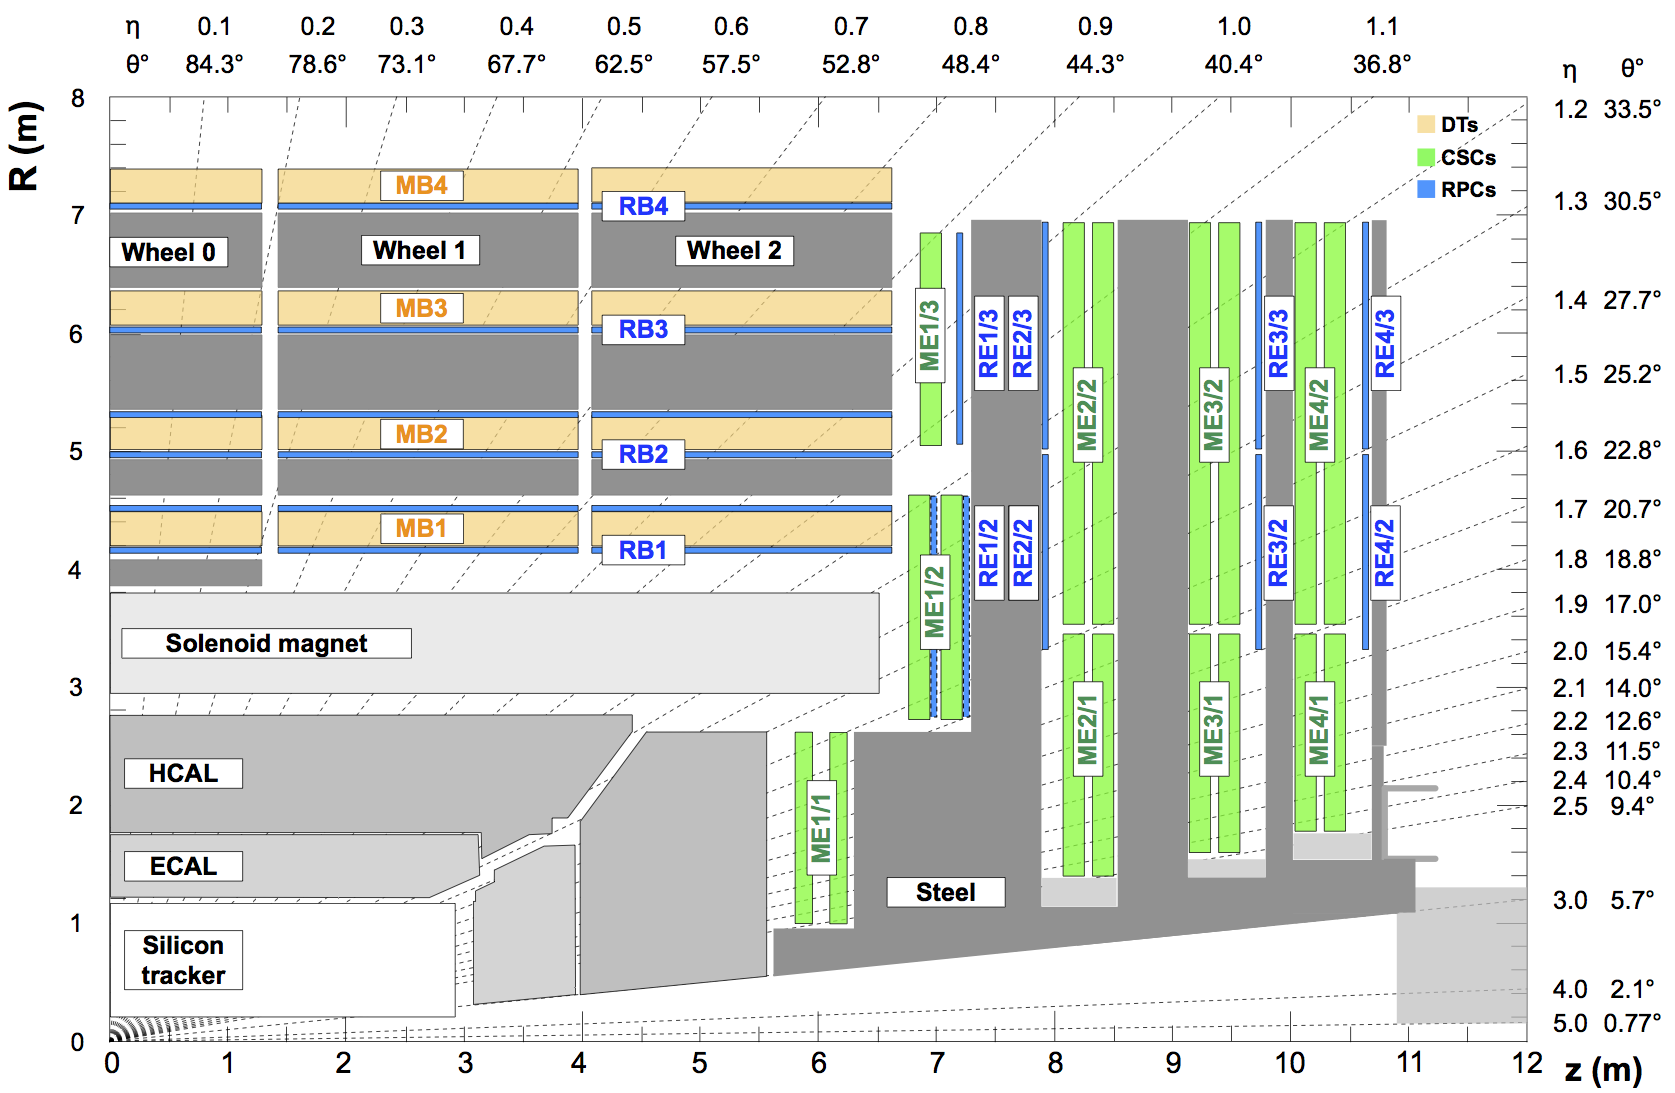
\includegraphics[width=0.9\textwidth]{plots/chapter3/muon.png}
  \caption{Schematic view of the muon detectors.}
  \label{fig:muon}
\end{figure}

\subsection{Trigger and data acquisition system}

The online event selection process, trigger, reduces the rate to about $1 \mathrm{KHz}$. The CMS experiment's trigger and data acquisition system is divided into four parts, summarised in Figure ?. First, the detector electronics detect signals and pass them to the Level-1 trigger processors. The Level-1 trigger logic is located in a service cavern and selects events of interest. Due to the size of the CMS detector and underground caverns, the transit and time needed for a decision is about 3.2 $\mu s$. However, the time needed for Level-1 trigger calculations is only 1 $\mu s$. At this time, the data is held in pipelined memory buffers.

Custom hardware processors form the Level-1 decision to keep or discard data using the calorimetry, muon systems, and correlation information. Trigger primitive objects, such as electrons or muons above a set \ET or \pt thresholds are used for the decision taking. Reduced granularity and resolution data are used to form the trigger objects. Sums of \ET and \met are also employed. Only about one out of 1000 interactions are retained. If the data of interaction is kept, the data is transferred after a fixed time interval of about $3.2 \mu s$ to the front-end readout buffers. The data is further processed and compressed, and placed in dual-port memories. A processor farm is responsible for filtering the events. Each processor runs the same High-Level Trigger (HLT) code, reducing the output rate from a few kHz to a few hundred Hz for mass storage. Using a processor farm for event filtering allows for computer technology evolution and maximizes the flexibility in selecting data and algorithms. Whenever possible, only necessary objects are reconstructed, and only needed information of some subdetectors are used. The idea of partial reconstruction and many virtual trigger levels is the basis for the HLT. First, calorimeter and muon information is used, followed by the use of pixel tracker data. Finally, the full event information is used, including full tracking. The HLT system uses identification and isolation criteria as well as minimal energy or transverse momentum thresholds.

\subsection{Luminosity measurement}

Luminosity L is defined as the ratio of the event rate $\dot{\mathrm{N}}$ to the cross-section $\sigma$ of a given process, and it is the effective area quantifying the likelihood of a scattering event.

\begin{equation}
  \mathcal{L}=\frac{\dot{\mathrm{N}}}{\sigma}
\end{equation}

The cross-section is measured in units of area, thus the luminosity is given in units of events per time per area, $(b.s)^{-1} = 10^{24} \lumi$. Then, the integrated luminosity L is the integral over the instantaneous luminosity:

\begin{equation}
  \mathrm{L}=\int \mathcal{L}(t) d t
\end{equation}

For a given process, the number of expected events which are produced is given by the product of the integrated luminosity and the production cross-section $\sigma_{exp}$:

\begin{equation}
  \mathrm{N_{exp}}=\mathrm{L} \cdot \sigma_{exp}
\end{equation}

Thus, the integrated luminosity has to be known to estimate the number of events for a given process or measure the production cross-section. Luminosity measurements are used to monitor the LHC performance in real-time, and they provide an overall normalization for physics analyses \cite{Bayatian:2006nff}. A reference process can be used to estimate the cross-section of a given process:

\begin{equation}
  \sigma_{\exp }=\frac{N_{\exp }}{N_{\text {ref }}} \cdot \sigma_{\text {ref }}
\end{equation}

where $N_{ref}$ and $\sigma_{ref}$ are the number of reference events and the reference process's cross-section. Furthermore, the same integrated luminosity has to be used for both processes. Colliders used nowadays employ bunched beams \cite{Tanabashi:2018oca}. If two bunches with $n_1$ and $n_2$ particles, respectively, collide head-on with frequency f, the instantaneous luminosity is given by:

\begin{equation}
\mathcal{L}=f \cdot \frac{n_{1} n_{2}}{\sqrt{\epsilon_{x} \beta_{x}^{*} \epsilon_{y} \beta_{y}^{*}}}
\end{equation}

where ${x,y}$ are the coordinates transverse to the beam, $\beta^*_{x,y}$ are the amplitude functions at the interaction point, where the beam optics produces a narrow focus. Emittance $\epsilon$ is a measure of the beam width defined as $\epsilon_{x} \equiv \frac{\sigma_{x}^{2}}{\beta_{x}}$, with $\sigma_{x}$ and $\sigma_{y}$ being the root mean square (RMS) of the transverse beam sizes in the horizontal or vertical direction, respectively. A high luminosity can be achieved with a high population of bunches of low emittance colliding at high frequency at locations where the beam optics provide low values of the amplitude functions. As the instantaneous luminosity depends on the beam parameters, it has to be measured when the beam parameter change. A reference process's event rate can estimate the instantaneous luminosity if the cross-section is known. The visible cross-section $\sigma_{vis}$ is given by:

\begin{equation}
  \sigma_{\mathrm{vis}}=\sigma(\mathrm{E}) \cdot \mathrm{A}(t, \mu, \ldots)
\end{equation}

where the cross-sections depend on the collision energy E and the detector acceptance A depends on time t, the mean number of interactions per bunch crossing $\mu$, and other parameters. Luminometers are independent detectors or parts of the detector for measuring the instantaneous luminosity. Once the calibration constant $\sigma_{vis}$ has been determined for a luminometer, the luminosity can be estimated using

\begin{equation}
  \mathcal{L}=\frac{\dot{\mathrm{N}}}{\sigma_{\mathrm{vis}}}
\end{equation}

where $\dot{\mathrm{N}}$ is the event rate for this luminometer. Ideally, the luminometer's visible cross-section should not be time-dependent and should not depend on experimental conditions. The visible cross-section has to be determined again when the beam parameters change. The same detector configuration has to be used during data-taking as during calibration. In summary, there are two important parts of the luminosity measurement. First, the luminometer, which measures the event rate. Secondly, the calibration of the luminometer. In the following, both parts of the luminosity measurement are introduced.

Luminometer: CMS uses five detectors to monitor and measure the luminosity based on rate measurements \cite{CMS:2019jhq, CMS:2018elu, CMS:2017sdi}. The CMS silicon pixel detector, the DTs in the muon system's barrel, the forward hadronic calorimeter, the Fast Beam Conditions Monitor (BCM1f), and the Pixel Luminosity Telescope (PLT) are used as luminometers. The luminometer of the pixel detector and the DTs use the standard CMS trigger and data acquisition system, while the PLT, BCM1f, and HF have an independent, fast readout system. However, the silicon pixel detector and the DT have very low occupancy and very good stability over time. In LHC Run I, only the silicon pixel detector and the HF were used as luminometers \cite{CMS:2013gfa}.

The HF has a high rate of acquisition, and it is most sensitive to the electromagnetic component of the hadronic showers. Two methods have been studied to estimate the luminosity. The first one, referred to as zero-counting, counts the hits above the single physical towers' threshold and averages each tower's result. The second method exploits the linear relationship between the total transverse energy deposit in the HF and the number of interactions and the luminosity. Both methods require that the mean value of interactions $\mu$ is proportional to the luminosity. The Pixel Cluster Counting (PCC) method employs a large number of pixels in the CMS detector. A given pixel has an exceedingly small probability of being hit by two different tracks from the same bunch crossing. For $\mu = 25$, the fraction of occupied pixels is less than a per mille. It is thus expected that the number of hit pixel clusters is a linear function of the number of interactions per crossing. Thus, the number of hit pixel clusters is a good measure of the instantaneous luminosity, which is given by:

\begin{equation}
  \mathcal{L}=\frac{\left\langle\mathrm{N}_{\text {cluster }}\right\rangle \cdot f}{\sigma_{\mathrm{vis}}^{\mathrm{PCC}}}
\end{equation}

where $\left\langle\mathrm{N}_{\text {cluster }}\right\rangle$ is the mean number of hit pixel clusters, f the orbit frequency of the LHC, and $\sigma_{vis}^{PCC}$ the visible cross-section of the PCC method. Pixel modules that have not been fully operational during calibration are omitted for the offline luminosity measurement. As the PCC method has a very small dependence on pileup and other experimental conditions, this method is chosen for the precision offline luminosity measurement. The HF measurements have a smaller statistical uncertainty and can be used for cross-checks or studies of the luminosity measurements' systematic uncertainties.

Van der Meer (VdM) scans: The whole cross-section is evaluated using Van der Meer (VdM) scans, which allows measuring the luminosity per colliding bunch pair from machine parameters. A counter system measures the counting rate proportional to the rate of the beam-beam interaction. One of the two beams is displaced, and the luminometer rate is measured as a function of the beam-beam separation resulting in a maximum at zero separation. The VdM scan method is used to assume that the two bunch densities factorize in x and y. These scans are performed with a dedicated LHC machine set up. Two beams are scanned through one another in the transverse plane of the detector. The luminosity and the luminosity rate must be determined at the same time to measure the visible cross-section:

\begin{equation}
  \sigma_{\mathrm{vis}}=2 \pi \Sigma_{x} \Sigma_{y}\langle n\rangle_{0}
\end{equation}

where $\Sigma_{x}$ and $\Sigma_{y}$ are the effective beam widths and $\langle n\rangle_{0}=\frac{1}{2}\left(\mathrm{R}_{x}+\mathrm{R}_{y}\right)$ with normalisation rates $R_x$ and $R_y$, which are the amplitudes of the fitted scan curves. Beam Imaging scans are used for studies on the beam shapes. The VdM scan also determines the transverse and longitudinal interaction point centroids.

Luminosity integration: After the VdM scan, the luminometer's visible cross-section is known, and the instantaneous luminosity can be measured. The integrated luminosity is obtained by summing the luminosities of short time intervals. The convenient minimal time interval to consider for the estimation of luminosity is the luminosity section (LS) corresponding to $t_{\mathrm{LS}}$ ($\sim 23$). The average number of clusters per event is computed for each LS, and the luminosity for the LS is derived and multiplied by $t_{\mathrm{LS}}$. The overall uncertainty on the luminosity measurement was between $2.3\%$ to $2.5\%$ for the three years. This is better than the design goal of a systematic accuracy of $5\%$.
